%
% Complete documentation on the extended LaTeX markup used for Insight
% documentation is available in ``Documenting Insight'', which is part
% of the standard documentation for Insight.  It may be found online
% at:
%
%     http://www.itk.org/

\documentclass{InsightArticle}

\usepackage[dvips]{graphicx}
\usepackage{subfigure}

%%%%%%%%%%%%%%%%%%%%%%%%%%%%%%%%%%%%%%%%%%%%%%%%%%%%%%%%%%%%%%%%%%
%
%  hyperref should be the last package to be loaded.
%
%%%%%%%%%%%%%%%%%%%%%%%%%%%%%%%%%%%%%%%%%%%%%%%%%%%%%%%%%%%%%%%%%%
\usepackage[dvips,
bookmarks,
bookmarksopen,
backref,
colorlinks,linkcolor={blue},citecolor={blue},urlcolor={blue},
]{hyperref}
\graphicspath{{fig/}}

\def \ie {\textit{i.e. }}
\def \etc {\textit{etc. }}
%  This is a template for Papers to the Insight Journal. 
%  It is comparable to a technical report format.

% The title should be descriptive enough for people to be able to find
% the relevant document. 
\title{Triangular Meshes Delaunay Conforming Filter}

% Increment the release number whenever significant changes are made.
% The author and/or editor can define 'significant' however they like.
\release{0.01}

% At minimum, give your name and an email address.  You can include a
% snail-mail address if you like.
\author{Arnaud Gelas, Alexandre Gouaillard\\
and Sean Megason}
\authoraddress{Department of System Biology, Harvard Medical School,\\
Boston, MA 02115, USA}

\begin{document}


\ifpdf
\else
   %
   % Commands for including Graphics when using latex
   % 
   \DeclareGraphicsExtensions{.eps,.jpg,.gif,.tiff,.bmp,.png}
   \DeclareGraphicsRule{.jpg}{eps}{.jpg.bb}{`convert #1 eps:-}
   \DeclareGraphicsRule{.gif}{eps}{.gif.bb}{`convert #1 eps:-}
   \DeclareGraphicsRule{.tiff}{eps}{.tiff.bb}{`convert #1 eps:-}
   \DeclareGraphicsRule{.bmp}{eps}{.bmp.bb}{`convert #1 eps:-}
   \DeclareGraphicsRule{.png}{eps}{.png.bb}{`convert #1 eps:-}
\fi


\maketitle


\ifhtml
\chapter*{Front Matter\label{front}}
\fi


% The abstract should be a paragraph or two long, and describe the
% scope of the document.
\begin{abstract}
\noindent
The \emph{Delaunay triangulation} is the triangulation of a set of points which maximizes the minimum angle of all angles of the triangles, and thus triangle aspect ratios. So converting a non Delaunay triangulation into a Delaunay triangulation, \emph{Delaunay conforming}, improves the all triangle aspect ratios and avoid elongated triangles. Note that combining this filter with usual operations like smoothing will provide a better approximation and a better distribution a triangle aspect ratios. Here this document describes a new filter based on the $n$D $2$-manifold mesh data structure available in itk: \code{itk::QuadEdgeMesh}~\cite{itkQE} to produce (planar or surfacic) Delaunay triangulation from any non-Delaunay triangulation by edge flipping, by implementing the edge flipping method decribed in~\cite{Dyer2007sgp}. 
\end{abstract}

\tableofcontents

\section{Introduction}
In the plane Delaunay triangulation of a set of points $\mathcal{P}$ is the triangulation such that no point $p$ of $\mathcal{P}$ is inside the circumcircle of any triangle of the triangulation. Such triangulations maximize the minimum angle of all angles of the triangles, and intend to avoid elongated triangles (see Figure~\ref{fig:results}).

Delaunay triangulations have been studied extensively in computational geometry first in $2$D, generalized in higher dimensions (in $3$D one Delaunay triangulation is a volumetric mesh where simplices are vertices, edges, triangles and tetraedrons), and for surface triangulation. Delaunay triangulations are nowadays used for many applications (simulation, finite-element analysis, visualization).

The filter presented here does not generate a Delaunay triangulation from a given set of points. Instead it creates a (planar or surfacic) Delaunay triangulation from a given $n$D $2$-manifold non-Delaunay triangulation by edge flipping without modifying the point locations, \ie only by changing the mesh connectivity, and under constraint of non exact geometry kernel.

\begin{figure}[ht]
  \centering
  \subfigure{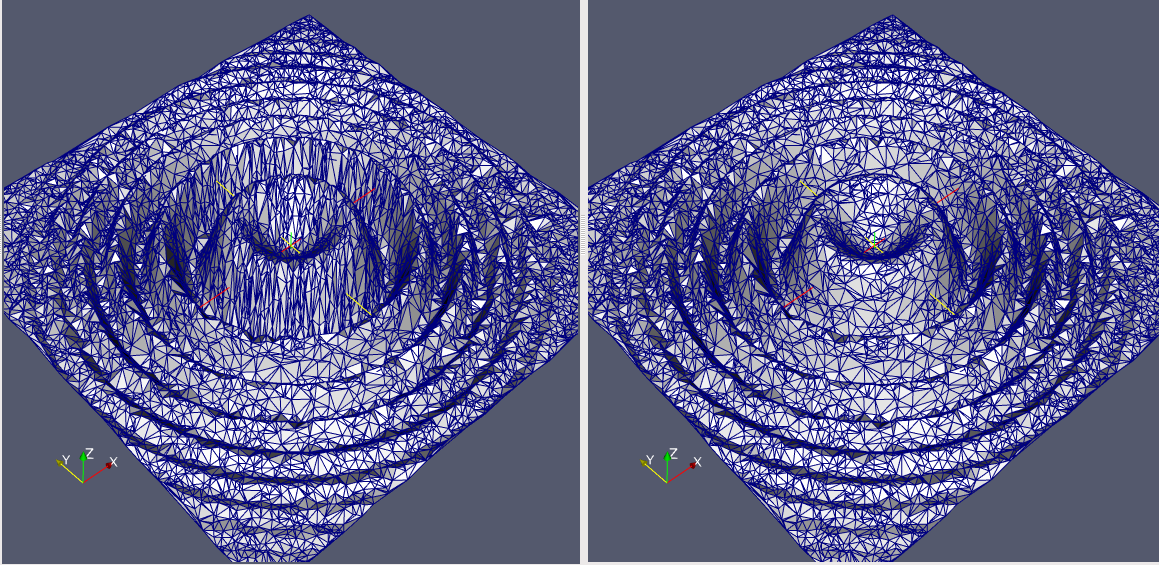
\includegraphics[width=0.9\textwidth]{wave0}}
  \subfigure{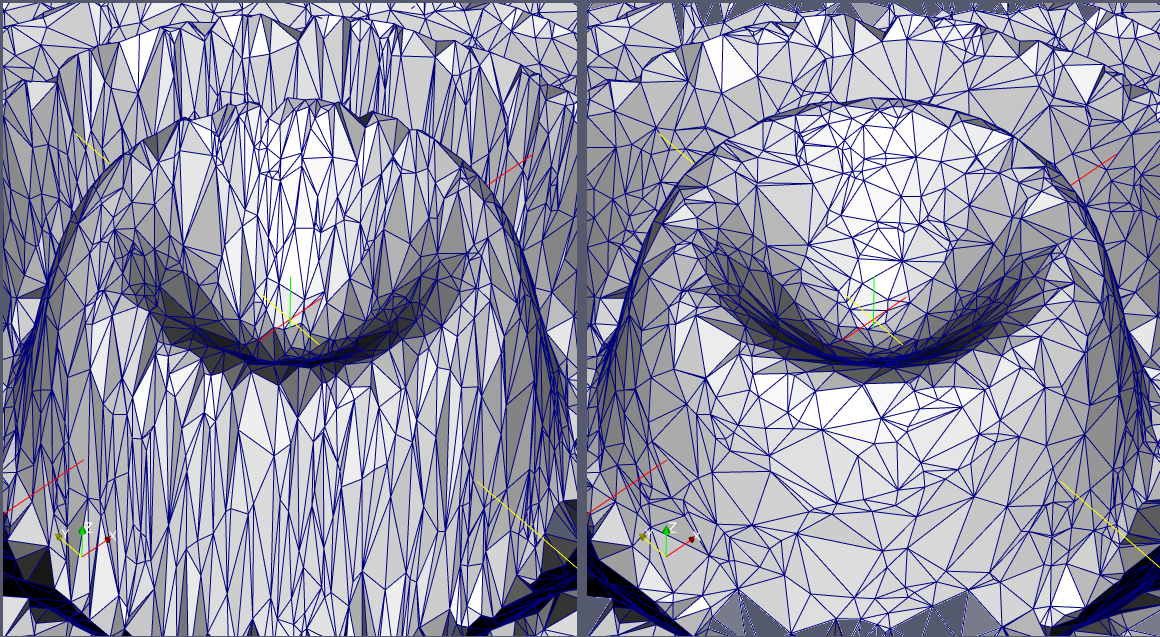
\includegraphics[width=0.9\textwidth]{wave1}}
  \caption{On the left a given non-Delaunay mesh $\mathcal{M}$, and on the right the resulting mesh after applying our filter.}
  \label{fig:results}
\end{figure}

\section{Principle}
Following~\cite{Dyer2007sgp}, we recall an \emph{unflippable edge} an edge such that its opposing edge also exists in the mesh, a \emph{constrained edge} is an edge which has been tagged by the user and which must not be modified\footnote{Constrained edge could be a boundary edge or a feature edge that the user wants to maintain.}, and thus a \emph{flippable edge} an edge which is not unflippable and not constrained.

Given a triangular mesh $\mathcal{M}$, all flippable edges are pushed into a priority queue. The priority $p(e)$ of a given edge $e$ is given by the sum of opposite angle (see Figure~\ref{fig:flip}):

\begin{equation}
  p(e) = \alpha + \beta - \pi \label{eq:flip}
\end{equation}

Then greedily the flippable edge $e$ with the largest priority is flipped, and the priority of edges next to $e$ is then updated. This process is reapeated until there is no more flippable edge with a positive priority in the priority queue.

\begin{figure}[t]
  \centering
  \subfigure[]{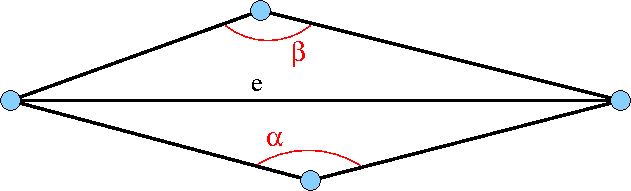
\includegraphics[width=0.4\textwidth]{flip0}}
  \hspace{2cm}
  \subfigure[]{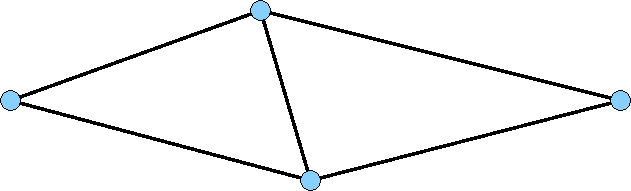
\includegraphics[width=0.4\textwidth]{flip1}}
  \caption{For a flippable edge $e$ we compute its priority $p(e)$ as the sum of opposite angles at $e$ minus $\pi$, \ie~$p = \alpha + \beta - \pi$~(a). If its priority is positive $e$ must be flipped~(b). The priority of the five edges displaid is then updated.}
  \label{fig:flip}
\end{figure}

\section{Implementation}
Based on the $n$D $2$-manifold mesh data structure (\code{itk::QuadEdgeMesh}~\cite{itkQE}), this filter is quite straightforward to implement. It only requires implementation of a method to compute the priority for a given edge~(see Eq.~\ref{eq:flip}), and a mutable priority queue container which allows to modify priority of any elements already inside the queue~\cite{itkPriorityQueueContainer}.

\section{Usage}

The use is really simple. The user only needs to provide a triangular mesh, and a list of constrained edges.

\begin{verbatim}
  typedef double Coord;
  const unsigned int Dimension = 3;
  typedef itk::QuadEdgeMesh< Coord, Dimension > MeshType;

  // Here we assume that mesh is given
  ...

  typedef itk::DelaunayConform< MeshType, MeshType > DelaunayConformFilterType;
  DelaunayConformFilterType::OutputEdgeCellListType list_of_constraints;
  
  // push here all constraints
  ...

  DelaunayConformFilterType::Pointer filter = DelaunayConformFilterType::New( );
  filter->SetInput( mesh );
  // if there is any constrained edges
  filter->SetListOfConstrainedEdges( list_of_constraints );
  filter->Update( );
\end{verbatim}

\section{Software Requirements}

You need to have the following software installed:

\begin{itemize}
  \item Insight Toolkit $\geq$ 3.7.0 (Revision $\geq$ 1.2737) compiled with USE\_REVIEW ON.
  \item CMake $\geq$ 2.4
\end{itemize}

\section*{Acknowledgement}
This work was funded by a grant from the NHGRI(P50HG004071-02) to found the Center for in toto genomic analysis of vertebrate development.

%%%%%%%%%%%%%%%%%%%%%%%%%%%%%%%%%%%%%%%%%
%
%  Insert the bibliography using BibTeX
%
%%%%%%%%%%%%%%%%%%%%%%%%%%%%%%%%%%%%%%%%%

\bibliographystyle{plain}
\bibliography{delaunay}


\end{document}

